\documentclass[11pt,a4paper]{report}

\usepackage[margin=2.5cm]{geometry}
\usepackage[T1]{fontenc}
\usepackage[utf8]{inputenc}
\usepackage{lmodern}
\usepackage{microtype}
\usepackage{xcolor}
\usepackage{graphicx}
\usepackage{amsmath,amssymb}
\usepackage{booktabs}
\usepackage{tabularx}
\usepackage{longtable}
\usepackage{array}
\usepackage{enumitem}
\usepackage{listings}
\usepackage{float}
\usepackage{tikz}
\usetikzlibrary{arrows.meta,positioning,shapes.geometric,fit,calc,decorations.pathreplacing}
\usepackage{fancyhdr}
\usepackage{titlesec}
\usepackage{hyperref}
\usepackage{caption}

\definecolor{PolimiBlue}{RGB}{0,83,155}
\definecolor{LightBlue}{RGB}{232,242,250}
\definecolor{LightGray}{RGB}{246,246,246}
\definecolor{MidGray}{RGB}{220,220,220}
\definecolor{DarkGray}{RGB}{70,70,70}
\definecolor{LightGreen}{RGB}{234,247,237}

\hypersetup{
  colorlinks=true,
  linkcolor=PolimiBlue,
  citecolor=PolimiBlue,
  urlcolor=PolimiBlue,
  pdftitle={Design Document - UAV Test Generator},
  pdfauthor={Roberto Capone and Guglielmo Cattaneo}
}

\setcounter{tocdepth}{3}
\setcounter{secnumdepth}{3}
\setlist[itemize]{leftmargin=1.6em,itemsep=2pt,topsep=4pt}
\setlist[enumerate]{leftmargin=1.8em,itemsep=2pt,topsep=4pt}
\renewcommand{\arraystretch}{1.18}
\newcolumntype{Y}{>{\raggedright\arraybackslash}X}
\newcolumntype{L}[1]{>{\raggedright\arraybackslash}p{#1}}

\pagestyle{fancy}
\fancyhf{}
\fancyhead[L]{UAV Test Generator -- Design Document}
\fancyhead[R]{Version 1.0}
\fancyfoot[C]{\thepage}
\setlength{\headheight}{14pt}

\titleformat{\chapter}[display]
  {\normalfont\bfseries\color{PolimiBlue}}
  {\filleft\Large\chaptertitlename\ \thechapter}
  {1ex}
  {\titlerule\vspace{1ex}\filright\Huge}

\lstset{
  language=Python,
  basicstyle=\ttfamily\small,
  backgroundcolor=\color{LightGray},
  frame=single,
  rulecolor=\color{black!20},
  breaklines=true,
  columns=fullflexible,
  keepspaces=true,
  showstringspaces=false,
  keywordstyle=\color{PolimiBlue}\bfseries,
  commentstyle=\color{DarkGray}\itshape
}

\newcommand{\projecttitle}{Search-Based Test Generation for Autonomous UAV Obstacle Avoidance Using a $(1+1)$-Evolution Strategy}
\newcommand{\systemname}{UAV Test Generator}
\newcommand{\code}[1]{\texttt{#1}}

\begin{document}

% ---------------------------------------------------------------------------
% Front page
% ---------------------------------------------------------------------------
\begin{titlepage}
\centering
\vspace*{1.5cm}
{\Large Politecnico di Milano\par}
\vspace{0.3cm}
{\large Software Engineering for Automation\par}
{\large A.Y. 2025--2026\par}
\vfill
{\Huge\bfseries\color{PolimiBlue} Design Document\par}
\vspace{0.8cm}
{\Large\bfseries \projecttitle\par}
\vfill
\begin{tabular}{rl}
\textbf{Authors:} & Roberto Capone\\
                  & Guglielmo Cattaneo\\[4pt]
\textbf{Instructor:} & Prof. Matteo Camilli\\[4pt]
\textbf{Version:} & 1.0\\
\textbf{Release date:} & 17/07/2026
\end{tabular}
\vfill
\end{titlepage}

\chapter*{Revision History}
\addcontentsline{toc}{chapter}{Revision History}
\begin{table}[H]
\centering
\begin{tabularx}{\textwidth}{L{2.2cm} L{2cm} L{4cm} Y}
\toprule
\textbf{Date} & \textbf{Version} & \textbf{Authors} & \textbf{Description}\\
\midrule
17/07/2026 & 1.0 & Roberto Capone; Guglielmo Cattaneo & Initial complete release aligned with the final \texttt{es-generator} implementation branch and Requirements Analysis and Specification version 1.0.\\
\bottomrule
\end{tabularx}
\end{table}

\tableofcontents
\clearpage

% ===========================================================================
\chapter{Introduction}
% ===========================================================================

\section{Purpose}
This document defines the architecture and detailed design of the \systemname. It translates the functional and non-functional requirements stated in the Requirements Analysis and Specification Document into components, classes, interfaces, algorithms, persistent data structures, runtime interactions, and integration decisions.

The design is descriptive of the final implementation in the \texttt{es-generator} branch. It therefore serves both as an architectural specification and as a traceability reference for reviewing the submitted source code.

\section{Project Goals}
The system is designed to generate effective and diverse failing test cases for PX4-Avoidance under a finite simulation budget. The principal design goals are:
\begin{itemize}
  \item preserve a simple competition-compatible command-line interface;
  \item separate deterministic search logic from expensive simulator interaction;
  \item enforce obstacle validity before simulation;
  \item use continuous failure severity to guide a $(1+1)$-Evolution Strategy;
  \item preserve diverse representative failures while retaining a complete persistent history;
  \item tolerate simulator non-determinism, timeouts, and process crashes;
  \item support reproducible experiments and a fair random-search baseline;
  \item produce inspectable and evaluator-ready output artifacts.
\end{itemize}

\section{Definitions, Acronyms, and Abbreviations}
The definitions from the Requirements Analysis and Specification Document apply. The following design-specific terms are used:
\begin{longtable}{L{3.4cm} L{11.4cm}}
\toprule
\textbf{Term} & \textbf{Definition}\\
\midrule
\endfirsthead
\toprule
\textbf{Term} & \textbf{Definition}\\
\midrule
\endhead
Pending candidate & Genes written to the checkpoint immediately before simulation so that an interrupted test can be repeated exactly.\\
Route corridor & Subset of the nominal trajectory used to guide obstacle placement and tune positional mutation scales.\\
Trajectory basin & Set of failures whose resampled trajectories are closer than the configured DTW threshold.\\
Trap gene & Additional obstacle targeted at the parent's observed escape gap and oriented across the local trajectory direction.\\
Delivery archive & Bounded in-memory list of representative failures used to construct the final suite; distinct from the complete persistent \texttt{all\_fails} history.\\
Variation point & Method deliberately overridden by \code{RandomGenerator} to replace evolutionary offspring creation with independent sampling.\\
\bottomrule
\end{longtable}

\section{Document Structure}
Chapter 2 presents the architectural design, including component, module, class, data, deployment, runtime, algorithmic, and pattern views. Chapter 3 specifies the command-line user interface and persistent output interface. Chapter 4 maps requirements to design elements and implementation files. Chapter 5 defines the implementation, integration, and test plan. Chapter 6 lists references.

% ===========================================================================
\chapter{Architectural Design}
% ===========================================================================

\section{Architectural Drivers}
The architecture is shaped by the following high-impact requirements:
\begin{enumerate}
  \item \textbf{Expensive and unstable execution.} Each simulator call may take several minutes, time out, or terminate the process; search state must therefore be persistent and simulation concerns isolated.
  \item \textbf{Strict global budget.} Every attempt must be accounted for before execution and no retry may bypass the limit.
  \item \textbf{External infrastructure.} PX4, Gazebo, and Aerialist are external dependencies accessed through a narrow wrapper.
  \item \textbf{Validity constraints.} Rotated boxes must fit within a legal region and must not overlap.
  \item \textbf{Multiple objectives with different roles.} Minimum distance guides the search, whereas simplicity, execution time, and diversity influence archive and delivery decisions.
  \item \textbf{Experimental comparability.} The evolutionary and random generators must share all infrastructure except the search mechanism.
  \item \textbf{Inspectable artifacts.} Every failure must be persistently represented as YAML and, when available, ULog and plot files.
\end{enumerate}

\section{Architecture Overview}
The system follows a modular pipeline architecture. The command-line layer selects and starts a generator. The generator coordinates mission handling, candidate production, execution, measurement, search-state transitions, archiving, checkpointing, and delivery. Deterministic geometry and scoring functions are isolated in a functional utility module. A small data model represents candidates independently of Aerialist objects. A test-case adapter encapsulates the external simulation API.

\begin{figure}[H]
\centering
\resizebox{\textwidth}{!}{%
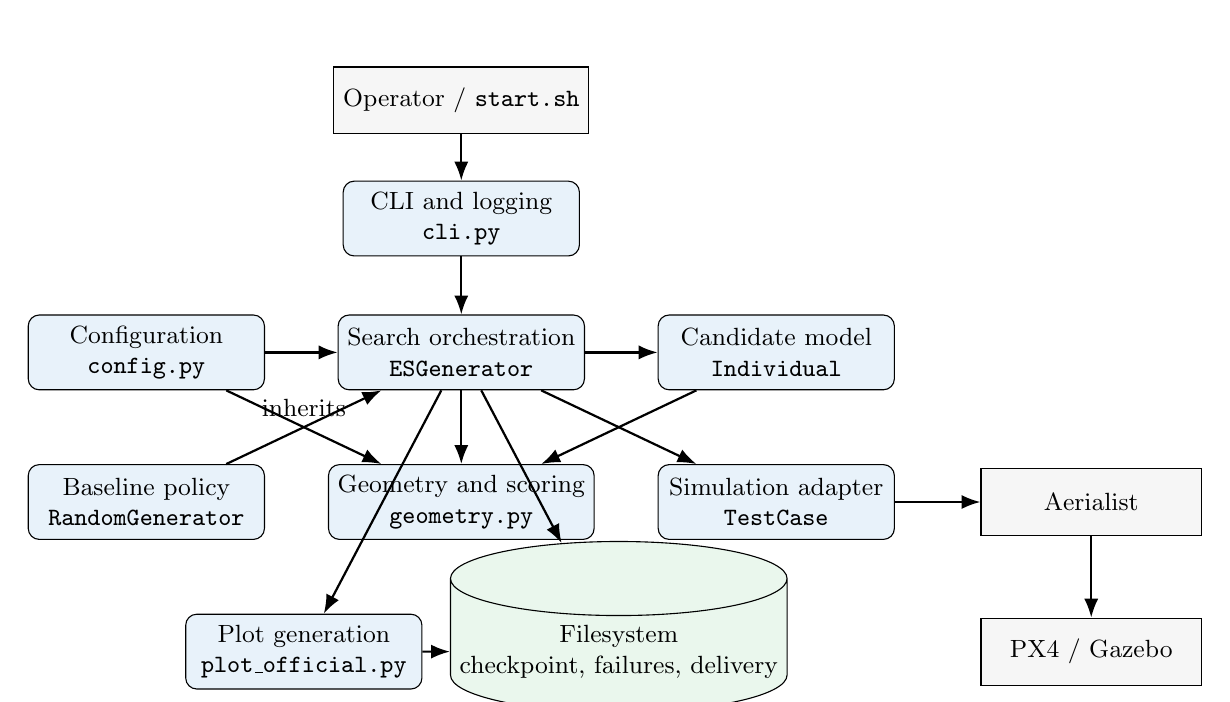
\begin{tikzpicture}[
 comp/.style={draw, rounded corners, align=center, minimum width=3.0cm, minimum height=0.95cm, fill=LightBlue},
 ext/.style={draw, align=center, minimum width=2.8cm, minimum height=0.85cm, fill=LightGray},
 data/.style={draw, cylinder, shape border rotate=90, aspect=0.22, align=center, minimum width=3.0cm, minimum height=0.95cm, fill=LightGreen},
 arr/.style={-{Latex[length=2.4mm]}, thick},
 font=\small
]
\node[ext] (launcher) at (6,4.0) {Operator / \code{start.sh}};
\node[comp] (cli) at (6,2.5) {CLI and logging\\\code{cli.py}};
\node[comp] (config) at (2,0.8) {Configuration\\\code{config.py}};
\node[comp] (gen) at (6,0.8) {Search orchestration\\\code{ESGenerator}};
\node[comp] (model) at (10,0.8) {Candidate model\\\code{Individual}};
\node[comp] (random) at (2,-1.1) {Baseline policy\\\code{RandomGenerator}};
\node[comp] (geom) at (6,-1.1) {Geometry and scoring\\\code{geometry.py}};
\node[comp] (tc) at (10,-1.1) {Simulation adapter\\\code{TestCase}};
\node[ext] (aerialist) at (14,-1.1) {Aerialist};
\node[comp] (plot) at (4,-3.0) {Plot generation\\\code{plot\_official.py}};
\node[data] (fs) at (8,-3.0) {Filesystem\\checkpoint, failures, delivery};
\node[ext] (sim) at (14,-3.0) {PX4 / Gazebo};

\draw[arr] (launcher) -- (cli);
\draw[arr] (cli) -- (gen);
\draw[arr] (config) -- (gen);
\draw[arr] (config) -- (geom);
\draw[arr] (random) -- node[above]{inherits} (gen);
\draw[arr] (gen) -- (model);
\draw[arr] (gen) -- (geom);
\draw[arr] (gen) -- (tc);
\draw[arr] (gen) -- (plot);
\draw[arr] (gen) -- (fs);
\draw[arr] (model) -- (geom);
\draw[arr] (tc) -- (aerialist);
\draw[arr] (aerialist) -- (sim);
\draw[arr] (plot) -- (fs);
\end{tikzpicture}%
}
\caption{Logical component view.}
\label{fig:components}
\end{figure}

\section{Component View}

\subsection{Command-Line and Logging Component}
\textbf{Implementation:} \code{cli.py}.

\textbf{Responsibilities:}
\begin{itemize}
  \item parse the \code{generate} operation, mission path, and budget;
  \item select \code{ESGenerator} or \code{RandomGenerator} through the \code{GENERATOR} environment variable;
  \item configure persistent and console logging;
  \item create the campaign output directory;
  \item invoke \code{generate()} and \code{write\_final\_selection()};
  \item convert uncaught exceptions into a logged non-zero process exit.
\end{itemize}

\textbf{Provided interface:}
\begin{lstlisting}[language=bash]
python3 cli.py generate <case-study.yaml> <budget>
\end{lstlisting}

\subsection{Configuration Component}
\textbf{Implementation:} \code{config.py}.

The configuration component centralises official bounds and environment-configurable parameters. Values are materialised at module import time. It also initialises Python's pseudo-random generator when \code{SEED} is present.

The principal parameter groups are:
\begin{itemize}
  \item legal obstacle dimensions and placement bounds;
  \item simulation timeout, retry, and repeated-evaluation parameters;
  \item adaptive route sampling and destination-completion parameters;
  \item mutation scale and stagnation parameters;
  \item archive size, spatial buckets, IoU, and DTW diversity parameters;
  \item trap-gene and intensification parameters.
\end{itemize}

\subsection{Candidate Model Component}
\textbf{Implementation:} \code{models.py}.

\code{Individual} is the central domain object. It owns only simple values or temporary references and therefore separates the generator's search state from the Aerialist execution model.

\begin{table}[H]
\centering
\begin{tabularx}{\textwidth}{L{3.4cm} L{3.0cm} Y}
\toprule
\textbf{Attribute} & \textbf{Type} & \textbf{Purpose}\\
\midrule
\code{genes} & list of lists & One to three genes $[l,w,h,x,y,r]$.\\
\code{fitness} & optional float & Search objective; minimum distance.\\
\code{min\_distance} & float & Most severe observed distance.\\
\code{completed} & bool & Whether the destination was reached with sufficient frequency.\\
\code{test\_case} & optional TestCase & In-memory best execution artifact; not checkpointed.\\
\code{fail\_base} & optional string & Relative base path of persistent failure files.\\
\code{avg\_point} & optional float & Mean competition point across executions.\\
\code{avg\_flight\_min} & optional float & Mean duration used by delivery ranking.\\
\code{traj} & optional list & Average resampled trajectory used for DTW.\\
\bottomrule
\end{tabularx}
\end{table}

The functions \code{\_ind\_to\_dict()} and \code{\_ind\_from\_dict()} define an explicit serialisation boundary. Aerialist objects are excluded, infinity is represented by \code{None}, and backward-compatible field fallbacks are supported.

\subsection{Geometry and Scoring Component}
\textbf{Implementation:} \code{geometry.py}.

This module contains pure or mostly pure functions for:
\begin{itemize}
  \item conversion from genes to Aerialist obstacles;
  \item rotated-box corner computation and overlap testing through the Separating Axis Theorem;
  \item rotation-aware fitting within legal bounds;
  \item route loading, destination detection, and destination reachability;
  \item random sampling, Gaussian mutation, and route-dependent step tuning;
  \item official point and ranking formulas;
  \item trajectory resampling and Dynamic Time Warping;
  \item non-overlapping obstacle generation, targeted trap-gene generation, and overlap repair.
\end{itemize}

Two module-level values, \code{\_ROUTE\_XY} and \code{\_DESTINATION}, represent campaign-specific route state. \code{GENE\_STEP} is mutable because its position entries are tuned to the loaded route.

\subsection{Simulation Adapter Component}
\textbf{Implementation:} \code{testcase.py}.

\code{TestCase} acts as an adapter around Aerialist. Its constructor deep-copies the immutable case study and replaces only the obstacle list. \code{execute()} selects the configured Aerialist agent, runs the test, and exposes the first returned trajectory and log file. \code{get\_distances()} delegates obstacle-distance measurement to the trajectory API. \code{save\_yaml()} serialises the enriched test description.

This component prevents the search controller from depending directly on local, Docker, or Kubernetes agent classes.

\subsection{Evolutionary Orchestration Component}
\textbf{Implementation:} \code{es\_generator.py}.

\code{ESGenerator} is the application service and state machine of the system. Its responsibilities are grouped as follows:
\begin{itemize}
  \item \textbf{evaluation:} retries, timeout, budget accounting, repeated executions, aggregation, completion assessment, and trajectory extraction;
  \item \textbf{route bootstrap:} obstacle-free simulation when no nominal route exists;
  \item \textbf{checkpointing:} atomic save and restoration of serialisable state;
  \item \textbf{search:} initial seeding, $(1+1)$ selection, mutation-scale adaptation, stagnation, restart, and intensification;
  \item \textbf{archive:} persistent failure dump, trajectory deduplication, bounded representative set, and replacement;
  \item \textbf{delivery:} score ordering, final DTW separation, idempotent copying, and stale-rank cleanup.
\end{itemize}

\subsection{Random Baseline Component}
\textbf{Implementation:} \code{random\_generator.py}.

\code{RandomGenerator} inherits \code{ESGenerator} and overrides two variation methods:
\begin{itemize}
  \item \code{\_make\_child()}, which returns an independently sampled one-obstacle individual;
  \item \code{\_restart\_individual()}, which also returns an independent sample.
\end{itemize}
Evaluation, validity, checkpointing, archive, delivery, and output formatting remain unchanged. This implements a controlled variation point: observed differences are attributable to the search policy rather than to different infrastructure.

\subsection{Plotting Component}
\textbf{Implementation:} \code{plot\_official.py}.

The plotter reads ULog data through \code{pyulog} when available and falls back to Aerialist trajectory extraction inside the container. It creates a composite figure with $x$, $y$, $z$, and yaw over time and a top-down map containing rotated obstacle rectangles and trajectory start/end markers. Plotting is deliberately non-critical: an exception is logged by the generator and does not terminate search.

\subsection{Launcher and Deployment Wrapper}
\textbf{Implementation:} \code{start.sh} and \code{Dockerfile}.

\code{start.sh} constructs a mission-specific output directory, cleans obsolete containers, mounts the source and output directories, copies generator files into the Aerialist working directory, starts one container for the whole budget, and restarts it after non-zero termination. The same output directory is reused so that the generator can restore its checkpoint. The wrapper also restores host file ownership.

The \code{Dockerfile} supports a self-contained image build by extending the Aerialist image, installing declared dependencies, copying the generator, creating output directories, and defining the default execution agent and PX4-Avoidance resources.

\section{Module Dependency View}
\begin{figure}[H]
\centering
\resizebox{\textwidth}{!}{%
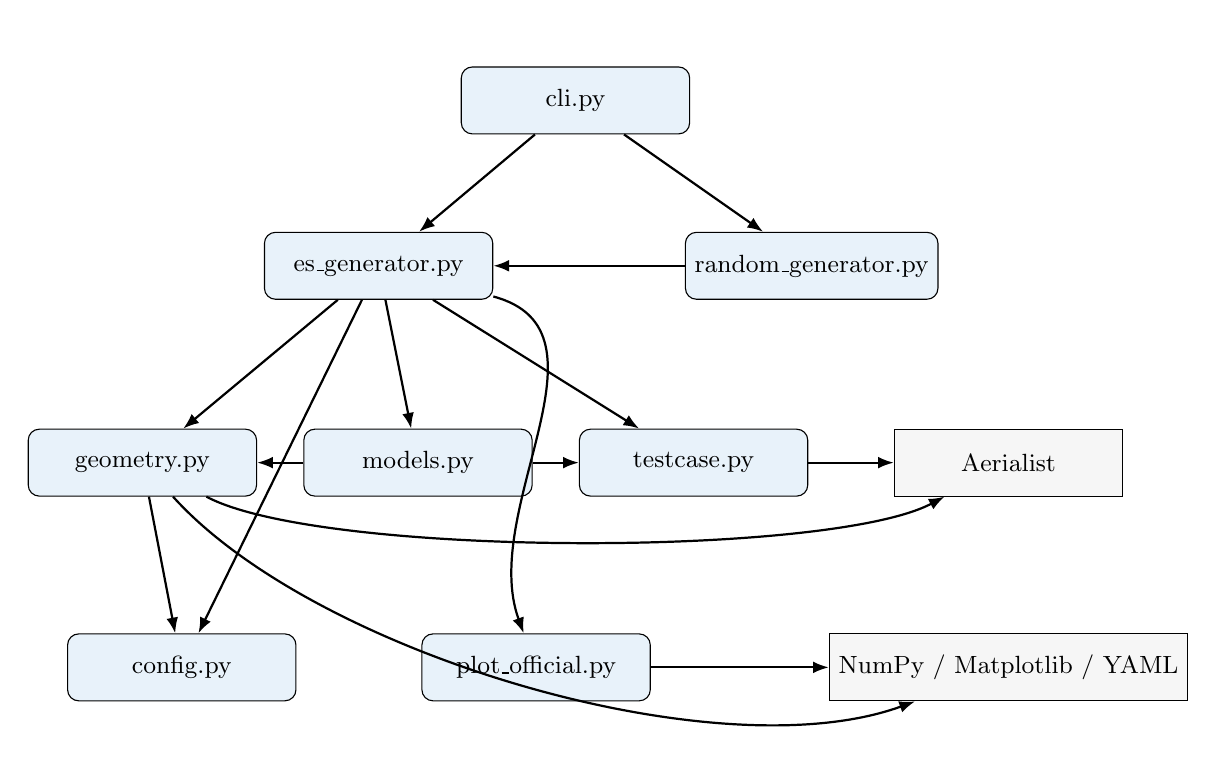
\begin{tikzpicture}[
 module/.style={draw, rounded corners, minimum width=2.9cm, minimum height=0.85cm, align=center, fill=LightBlue},
 external/.style={draw, minimum width=2.9cm, minimum height=0.85cm, align=center, fill=LightGray},
 dep/.style={-{Latex[length=2mm]}, thick},
 font=\small
]
\node[module]   (cli)       at (5,4.6)     {cli.py};
\node[module]   (es)        at (2.5,2.5)   {es\_generator.py};
\node[module]   (random)    at (8,2.5)     {random\_generator.py};
\node[module]   (geom)      at (-0.5,0)    {geometry.py};
\node[module]   (model)     at (3,0)       {models.py};
\node[module]   (tc)        at (6.5,0)     {testcase.py};
\node[external] (aerialist) at (10.5,0)    {Aerialist};
\node[module]   (config)    at (0,-2.6)    {config.py};
\node[module]   (plot)      at (4.5,-2.6)  {plot\_official.py};
\node[external] (libs)      at (10.5,-2.6) {NumPy / Matplotlib / YAML};

\draw[dep] (cli) -- (es);
\draw[dep] (cli) -- (random);
\draw[dep] (random) -- (es);
\draw[dep] (es) -- (geom);
\draw[dep] (es) -- (model);
\draw[dep] (es) -- (tc);
\draw[dep] (es) -- (config);
\draw[dep] (es) to[out=-15,in=110] (plot);
\draw[dep] (model) -- (geom);
\draw[dep] (model) -- (tc);
\draw[dep] (geom) -- (config);
\draw[dep] (geom) to[out=-28,in=208,looseness=0.45] (aerialist);
\draw[dep] (tc) -- (aerialist);
\draw[dep] (plot) -- (libs);
\draw[dep] (geom) to[out=-48,in=200,looseness=0.7] (libs);
\end{tikzpicture}%
}
\caption{Static module dependencies.}
\label{fig:modules}
\end{figure}

\section{Class View}
\begin{figure}[H]
\centering
\resizebox{\textwidth}{!}{%
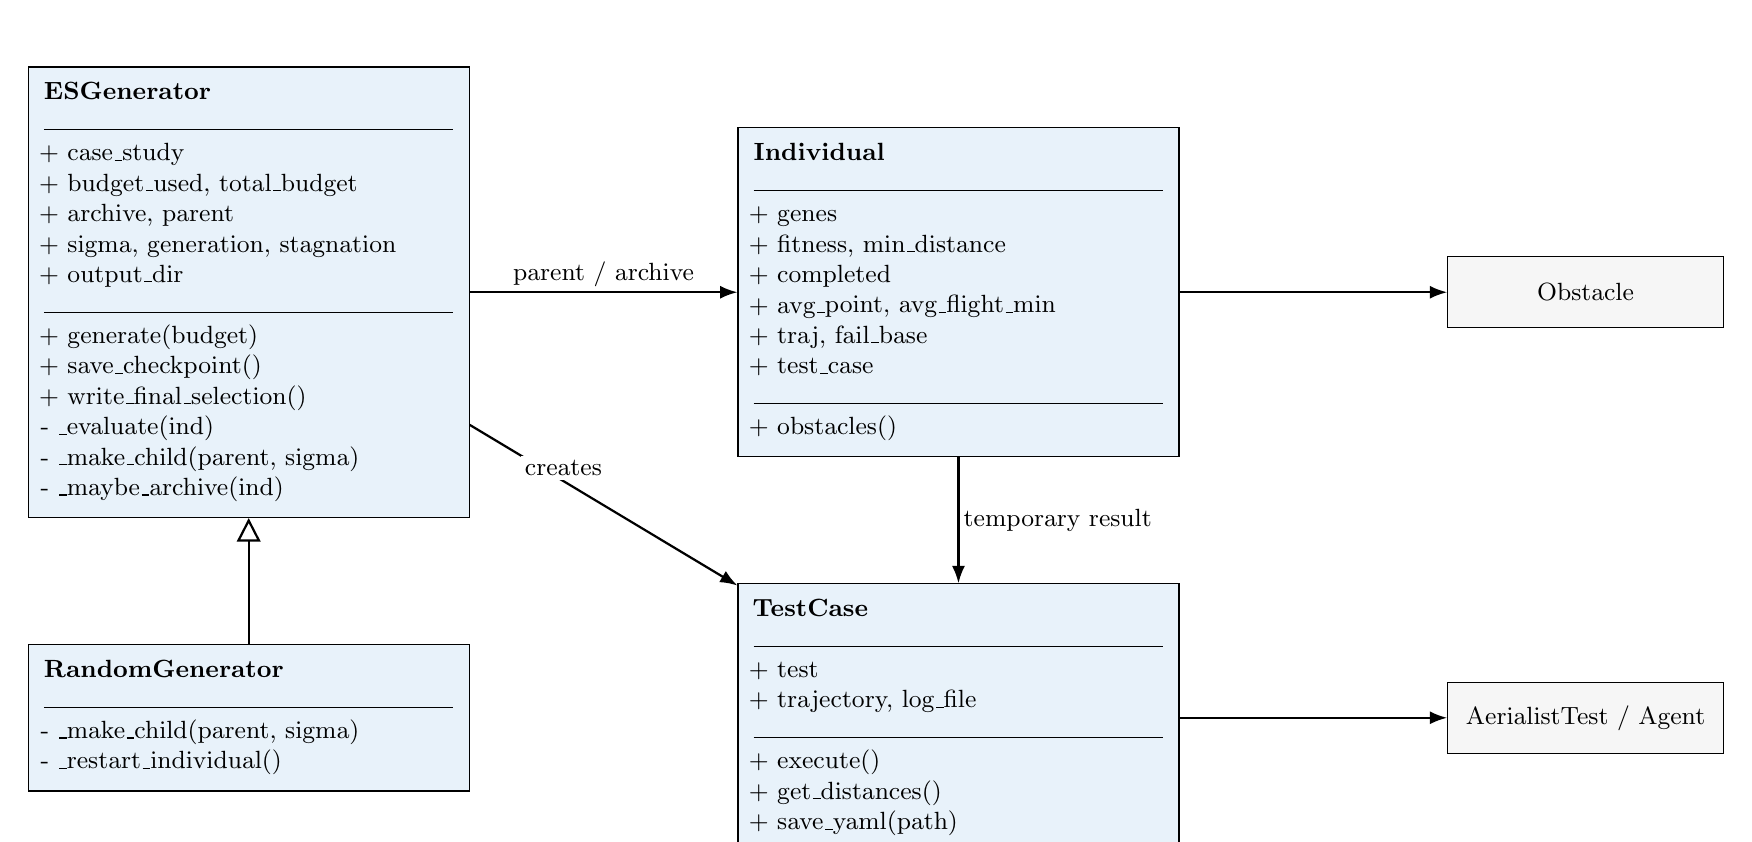
\begin{tikzpicture}[
 cls/.style={draw, rectangle, align=left, text width=5.2cm, inner sep=2mm, fill=LightBlue},
 ext/.style={draw, rectangle, align=center, minimum width=3.5cm, minimum height=0.9cm, fill=LightGray},
 inherit/.style={-{Triangle[open,length=3mm,width=3mm]}, thick},
 assoc/.style={-{Latex[length=2.2mm]}, thick},
 lbl/.style={fill=white, inner sep=1.5pt},
 node distance=16mm and 34mm,
 font=\small
]
\node[cls] (es) {\textbf{ESGenerator}\\\hrulefill\\
+ case\_study\\+ budget\_used, total\_budget\\+ archive, parent\\+ sigma, generation, stagnation\\+ output\_dir\\\hrulefill\\
+ generate(budget)\\+ save\_checkpoint()\\+ write\_final\_selection()\\- \_evaluate(ind)\\- \_make\_child(parent, sigma)\\- \_maybe\_archive(ind)};

\node[cls, right=of es] (ind) {\textbf{Individual}\\\hrulefill\\
+ genes\\+ fitness, min\_distance\\+ completed\\+ avg\_point, avg\_flight\_min\\+ traj, fail\_base\\+ test\_case\\\hrulefill\\
+ obstacles()};

\node[cls, below=of es] (rand) {\textbf{RandomGenerator}\\\hrulefill\\
- \_make\_child(parent, sigma)\\- \_restart\_individual()};

\node[cls, below=of ind] (tc) {\textbf{TestCase}\\\hrulefill\\
+ test\\+ trajectory, log\_file\\\hrulefill\\
+ execute()\\+ get\_distances()\\+ save\_yaml(path)};

\node[ext, right=of tc] (air) {AerialistTest / Agent};
\node[ext, right=of ind] (obs) {Obstacle};

\draw[inherit] (rand) -- (es);
\draw[assoc] (es) -- node[above,lbl]{parent / archive} (ind);
\draw[assoc] (es) -- node[above,lbl,pos=0.35]{creates} (tc);
\draw[assoc] (ind) -- node[right,lbl]{temporary result} (tc);
\draw[assoc] (ind) -- (obs);
\draw[assoc] (tc) -- (air);
\end{tikzpicture}%
}
\caption{Principal class relationships. Utility functions in \code{geometry.py} and constants in \code{config.py} are not represented as artificial classes.}
\label{fig:classes}
\end{figure}

\section{Data Design}

\subsection{Obstacle Genome}
A candidate genome is a list
\[
G=\left[g_1,\ldots,g_n\right],\qquad 1\le n\le 3,
\]
where
\[
g_i=[l_i,w_i,h_i,x_i,y_i,r_i].
\]
The vertical position is not stored because it is fixed to $z_i=0$. Gene-to-obstacle conversion occurs only when the candidate is prepared for execution or geometric comparison.

\subsection{Checkpoint Schema}
The checkpoint is a JSON object containing:
\begin{itemize}
  \item budget and run metadata: \code{budget\_used}, \code{total\_budget}, and seed;
  \item search state: \code{sigma}, generation, stagnation, success history;
  \item crash state: pending genes;
  \item initialisation state: seeding flag, remaining seeds, and best seed;
  \item parent and serialised archive individuals;
  \item route and destination state.
\end{itemize}

The write protocol is:
\begin{enumerate}
  \item serialise to \code{checkpoint.json.tmp};
  \item close the temporary file;
  \item atomically replace \code{checkpoint.json} using \code{os.replace()}.
\end{enumerate}
This prevents a process failure during writing from destroying the previous valid snapshot.

\subsection{Persistent Output Layout}
\begin{lstlisting}[language={}]
generated_tests/<mission>-<generator>[-sSEED]-<date>/
|-- checkpoint.json
|-- debug.txt
|-- all_fails/
|   |-- fail_d<distance>_obs<count>_run<budget>.yaml
|   |-- fail_d<distance>_obs<count>_run<budget>.ulg
|   `-- fail_d<distance>_obs<count>_run<budget>_plot.png
`-- consegna/
    |-- rank01_d<distance>_obs<count>.yaml
    |-- rank01_d<distance>_obs<count>.ulg
    `-- rank01_d<distance>_obs<count>_plot.png
\end{lstlisting}

The complete failure history is append-only from the perspective of delivery construction. Delivery files are copies; they may be rebuilt or stale ranks removed without altering \code{all\_fails}.

\section{Runtime View}

\subsection{Fresh Evolutionary Run}
\begin{figure}[H]
\centering
\resizebox{\textwidth}{!}{%
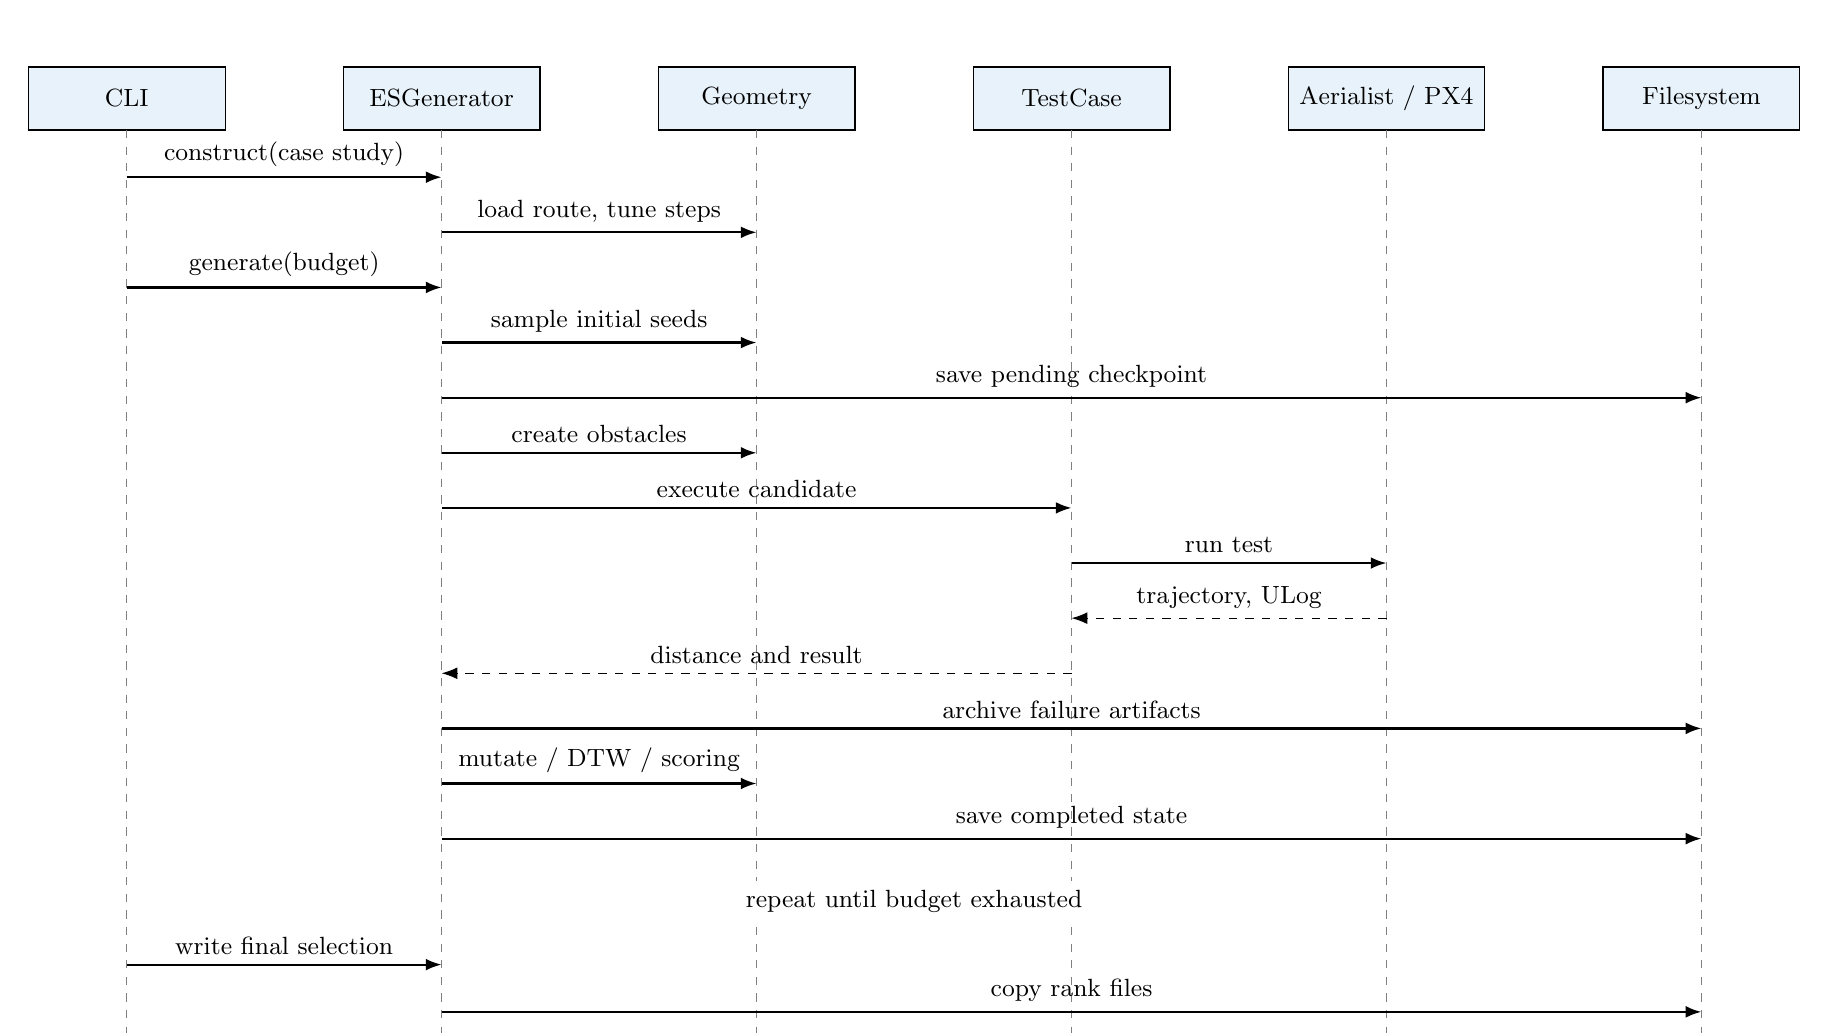
\begin{tikzpicture}[
 lifeline/.style={draw, fill=LightBlue, minimum width=2.5cm, minimum height=0.8cm, align=center},
 msg/.style={-{Latex[length=2mm]}, thick},
 ret/.style={-{Latex[length=2mm]}, dashed},
 font=\small
]
\node[lifeline] (cli) at (0,0) {CLI};
\node[lifeline] (gen) at (4,0) {ESGenerator};
\node[lifeline] (geo) at (8,0) {Geometry};
\node[lifeline] (tc) at (12,0) {TestCase};
\node[lifeline] (sim) at (16,0) {Aerialist / PX4};
\node[lifeline] (fs) at (20,0) {Filesystem};
\foreach \x in {0,4,8,12,16,20} {\draw[dashed,gray] (\x,-0.4) -- (\x,-12.0);}

\draw[msg] (0,-1) -- node[above]{construct(case study)} (4,-1);
\draw[msg] (4,-1.7) -- node[above]{load route, tune steps} (8,-1.7);
\draw[msg] (0,-2.4) -- node[above]{generate(budget)} (4,-2.4);
\draw[msg] (4,-3.1) -- node[above]{sample initial seeds} (8,-3.1);
\draw[msg] (4,-3.8) -- node[above]{save pending checkpoint} (20,-3.8);
\draw[msg] (4,-4.5) -- node[above]{create obstacles} (8,-4.5);
\draw[msg] (4,-5.2) -- node[above]{execute candidate} (12,-5.2);
\draw[msg] (12,-5.9) -- node[above]{run test} (16,-5.9);
\draw[ret] (16,-6.6) -- node[above]{trajectory, ULog} (12,-6.6);
\draw[ret] (12,-7.3) -- node[above]{distance and result} (4,-7.3);
\draw[msg] (4,-8.0) -- node[above]{archive failure artifacts} (20,-8.0);
\draw[msg] (4,-8.7) -- node[above]{mutate / DTW / scoring} (8,-8.7);
\draw[msg] (4,-9.4) -- node[above]{save completed state} (20,-9.4);
\node[fill=white,align=center] at (10,-10.2) {repeat until budget exhausted};
\draw[msg] (0,-11.0) -- node[above]{write final selection} (4,-11.0);
\draw[msg] (4,-11.6) -- node[above]{copy rank files} (20,-11.6);
\end{tikzpicture}%
}
\caption{Fresh-run sequence.}
\label{fig:freshseq}
\end{figure}

\subsection{Crash and Resume}
Before every candidate evaluation, the controller records the candidate genes as \code{pending}. If the process terminates during the simulator call, the checkpoint still references that candidate. \code{start.sh} re-enters the same output directory, the generator restores the checkpoint, reconstructs an \code{Individual} from the pending genes, and executes the full candidate again. Partial simulator state is never reused.

This design establishes the following recovery invariant:
\begin{quote}
At any restart point, all failures completed before the most recently pending candidate are persistent, and the next semantically valid action is to repeat that pending candidate from the beginning.
\end{quote}

\subsection{Final Delivery Construction}
The controller sorts the archive by delivery score. It greedily scans the sorted list and retains a candidate only when its trajectory is sufficiently separated from every already retained trajectory. For each retained individual, the controller copies available \code{.yaml}, \code{.ulg}, and \code{\_plot.png} files from \code{all\_fails} to \code{consegna} using a rank-prefixed basename. A cleanup pass removes only delivery files whose base names are no longer expected.

\section{Algorithm Design}

\subsection{Search Fitness}
For an execution trajectory $\tau$ and obstacle set $O$, let $d(\tau,o)$ be the minimum trajectory-to-obstacle distance. The candidate fitness is
\[
f(G)=\min_{o\in O} d(\tau,o).
\]
When a candidate is executed multiple times, the implementation uses the minimum observed distance as fitness:
\[
f(G)=\min_{k\in\{1,\ldots,m\}}\min_{o\in O}d(\tau_k,o).
\]
Selection is strict minimisation. The number of obstacles is deliberately excluded from fitness so that the search does not trade a less severe failure for simplicity prematurely.

\subsection{Initialisation}
In adaptive mode, obstacle centres are sampled around a randomly chosen point of the nominal route:
\[
x=x_{\mathrm{route}}+\varepsilon_x,\qquad
 y=y_{\mathrm{route}}+\varepsilon_y,
\]
with Gaussian jitter followed by clamping and rotation-aware fitting. A configurable number of single-obstacle seeds is evaluated. The seed with minimum fitness becomes the first parent.

\subsection{Gaussian Mutation}
Each gene coordinate is mutated independently:
\[
g_i'=\operatorname{clamp}\left(g_i+\mathcal{N}\left(0,\sigma^2 s_i^2\right),\;g_i^{\min},\;g_i^{\max}\right),
\]
where $s_i$ is a dimension-specific step scale and $\sigma$ is the global mutation scale. Position scales are derived from the route extent and bounded by configurable minimum and maximum values. After mutation, obstacle centres are corrected so that the complete rotated boxes remain legal.

The offspring operator may also:
\begin{itemize}
  \item add an obstacle when fewer than three are present;
  \item remove a random obstacle when more than one is present;
  \item repair overlaps by retaining the first obstacle and discarding later overlapping obstacles.
\end{itemize}

\subsection{Mutation-Scale Adaptation}
The implementation applies Rechenberg's $1/5$ success rule over a bounded recent window. Let
\[
p_s=\frac{1}{w}\sum_{j=1}^{w} I_j,
\]
where $I_j=1$ when the child strictly improved the parent and $0$ otherwise. The scale update is
\[
\sigma'=
\begin{cases}
\min(1.22\sigma,\sigma_{\max}), & p_s>0.2,\\[2mm]
\max(\sigma/1.22,\sigma_{\min}), & p_s\le 0.2.
\end{cases}
\]
The scale is unchanged until the success-history window is full.

\subsection{Trap-Gene Operator}
When a new obstacle is added and a parent trajectory is available, the trap operator may replace pure random insertion.

For every trajectory point, the algorithm measures its distance to the existing obstacles and chooses the point closest to them. This point represents the gap through which the UAV escaped. A discrete local tangent estimates the direction of motion. The proposed obstacle is oriented approximately perpendicular to this direction. Its long side is proportional to the measured gap, bounded by the legal dimension range and an explicit cap. Gaussian position jitter prevents identical insertions. The candidate is accepted only if it does not overlap existing obstacles.

\subsection{Stagnation and Restart}
The stagnation counter increases after every non-improving child and receives an additional increment for a redundant failure. Once the threshold is reached, the generator replaces the parent and resets the mutation scale.

A diversified restart partitions the legal $y$ interval into buckets. It prefers an uncovered bucket and generates several candidate genes, selecting the one with minimum maximum IoU against archived obstacles. When every bucket is represented, the generator may intensify around the most severe archived failure by copying its genes and, if possible, adding a trap gene.

\subsection{Failure Point and Delivery Score}
For a simulation with minimum distance $d$, the point value is
\[
p(d)=
\begin{cases}
5, & d<0.25,\\
2, & 0.25\le d<1.0,\\
1, & 1.0\le d<1.5,\\
0, & d\ge 1.5.
\end{cases}
\]
For a test case $t$, the delivery score is
\[
S(t)=\frac{10\,\overline{p}(t)}{n_{\mathrm{obs}}(t)^2\,\overline{T}(t)},
\]
where $\overline{T}$ is clamped away from zero to avoid numerical blow-up. This score is used only for archive eviction and final ordering.

\subsection{Trajectory Representation and DTW}
A successful trajectory is resampled to a fixed number $N$ of $(x,y)$ points. When repeated executions are available, corresponding samples are averaged.

For trajectories $A=(a_1,\ldots,a_n)$ and $B=(b_1,\ldots,b_m)$, the dynamic-programming recurrence is
\[
D_{i,j}=\lVert a_i-b_j\rVert_2+
\min\{D_{i-1,j},D_{i,j-1},D_{i-1,j-1}\},
\]
with $D_{0,0}=0$ and unreachable boundary cells set to infinity. The final value is normalised by the backtracked alignment length, yielding a mean deviation in metres.

Two failures belong to the same trajectory basin when their DTW distance is below \code{DTW\_THRESHOLD}. When trajectory data are unavailable, geometric IoU is used as a fallback.

\subsection{Archive Policy}
For every failure $f(G)<1.5$:
\begin{enumerate}
  \item save its artifacts immediately to \code{all\_fails};
  \item search the archive for the closest trajectory basin;
  \item if a duplicate basin exists, retain only the candidate with lower minimum distance as the in-memory representative;
  \item if no duplicate exists and capacity is available, append it;
  \item if capacity is full, replace the lowest delivery-score entry only when the new candidate has a higher score.
\end{enumerate}

This separates complete evidence preservation from bounded evaluator-facing selection.

\section{Error Handling and Fault Tolerance}
\begin{table}[H]
\centering
\begin{tabularx}{\textwidth}{L{4cm} Y Y}
\toprule
\textbf{Failure mode} & \textbf{Local handling} & \textbf{Persistent effect}\\
\midrule
Simulation timeout & Cancel alarm, log warning, retry if budget and retry count permit. & Attempt remains counted; checkpoint still protects the candidate.\\
Aerialist execution exception & Log compact diagnostic and retry. & Attempt remains counted.\\
Container/process crash & External wrapper restarts container. & Last valid checkpoint and previously dumped failures remain.\\
Interrupted candidate & Reconstruct from pending genes and repeat from start. & No partial simulation is treated as a valid result.\\
Unreadable checkpoint & Log warning and use documented clean-start behaviour. & Existing failure files are not deleted.\\
Missing nominal ULog & Attempt route bootstrap; otherwise fixed sampling region. & Route fallback is reflected in logs and checkpoint.\\
Missing trajectory metadata & Use neutral or geometric fallbacks for completion, time, or similarity. & Candidate may remain usable.\\
Plotting failure & Log warning and continue. & YAML and ULog remain deliverable.\\
File-copy failure & Log rank-specific warning and continue with remaining ranks. & Source failure files remain in \code{all\_fails}.\\
User interruption & Launcher disables restart loop and terminates. & Checkpoint and failure history remain available.\\
\bottomrule
\end{tabularx}
\end{table}

\section{Deployment View}
\begin{figure}[H]
\centering
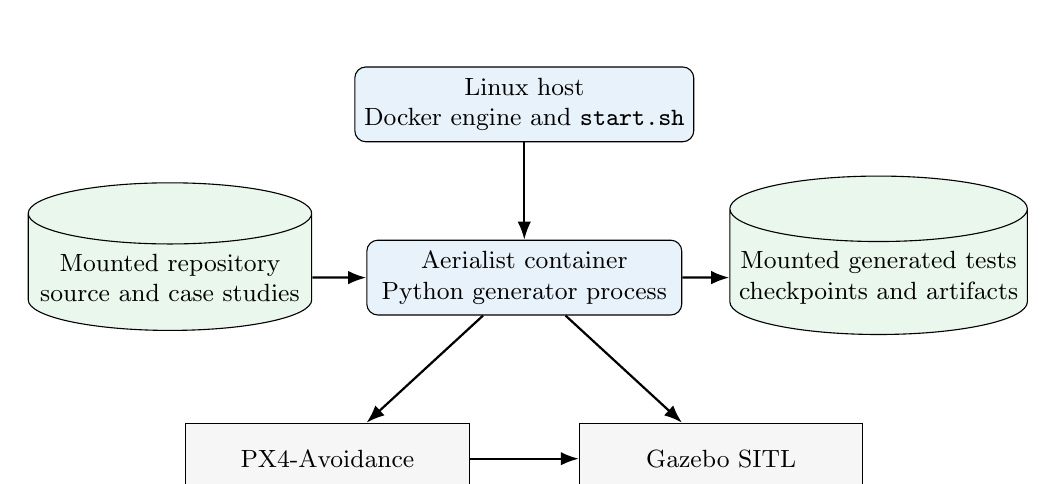
\begin{tikzpicture}[
 nodebox/.style={draw, rounded corners, align=center, minimum width=4.0cm, minimum height=0.95cm, fill=LightBlue},
 ext/.style={draw, align=center, minimum width=3.6cm, minimum height=0.9cm, fill=LightGray},
 store/.style={draw, cylinder, shape border rotate=90, aspect=0.22, align=center, minimum width=3.6cm, minimum height=1.0cm, fill=LightGreen},
 arr/.style={-{Latex[length=2.3mm]}, thick},
 font=\small
]
\node[nodebox] (host) at (6,3.2) {Linux host\\Docker engine and \code{start.sh}};
\node[store] (repo) at (1.5,1.0) {Mounted repository\\source and case studies};
\node[nodebox] (container) at (6,1.0) {Aerialist container\\Python generator process};
\node[store] (out) at (10.5,1.0) {Mounted generated tests\\checkpoints and artifacts};
\node[ext] (px4) at (3.5,-1.3) {PX4-Avoidance};
\node[ext] (gazebo) at (8.5,-1.3) {Gazebo SITL};

\draw[arr] (host) -- (container);
\draw[arr] (repo) -- (container);
\draw[arr] (container) -- (out);
\draw[arr] (container) -- (px4);
\draw[arr] (container) -- (gazebo);
\draw[arr] (px4) -- (gazebo);
\end{tikzpicture}
\caption{Reference Docker deployment.}
\label{fig:deployment}
\end{figure}

\section{Architectural Styles and Patterns}

\subsection{Modular / Layered Organisation}
The code separates interface, orchestration, domain model, deterministic domain services, infrastructure adapter, and presentation concerns. The separation is pragmatic rather than enforced by a framework, but dependencies predominantly point inward toward simple model and geometry logic.

\subsection{Strategy Variation through Inheritance}
\code{RandomGenerator} is substitutable for \code{ESGenerator} at the CLI boundary. The candidate-generation and restart methods are variation points, whereas the expensive common infrastructure is inherited. This resembles the Strategy and Template Method patterns: \code{generate()} defines the invariant process, and selected protected methods define the varying policy.

\subsection{Adapter}
\code{TestCase} adapts the Aerialist execution API to the generator's needs. It hides agent selection and exposes a minimal interface: execute, obtain distances, and save YAML.

\subsection{Checkpoint / Memento}
The checkpoint is an explicit serialisable snapshot of the generator's logical state. It resembles the Memento pattern while avoiding opaque object serialisation. The generator remains responsible for producing and restoring the memento.

\subsection{Repository-Like Failure Store}
The filesystem-backed \code{all\_fails} directory provides durable append-style storage, while the in-memory archive provides a bounded set of representatives. The distinction avoids coupling evidence retention to evaluator capacity.

\subsection{Functional Core, Imperative Shell}
Geometry, scoring, DTW, mutation, and serialisation are implemented as testable functions. The stateful \code{ESGenerator} forms an imperative shell that sequences simulator and filesystem effects. This separation improves testability and reduces the scope of failure-prone code.

\section{Design Decisions and Trade-Offs}
\begin{longtable}{L{4cm} L{5.2cm} L{5.2cm}}
\toprule
\textbf{Decision} & \textbf{Benefit} & \textbf{Trade-off}\\
\midrule
\endfirsthead
\toprule
\textbf{Decision} & \textbf{Benefit} & \textbf{Trade-off}\\
\midrule
\endhead
Minimum distance as search fitness & Continuous gradient-like signal; directly targets safety severity. & Ignores obstacle simplicity during search; handled later by ranking.\\
One parent and one child & Small state, simple checkpointing, efficient under expensive simulations. & Less population diversity than larger evolutionary algorithms.\\
Adaptive route sampling & Concentrates evaluations in mission-relevant regions. & Requires a nominal log or one budget-consuming bootstrap.\\
Route-dependent mutation scale & Prevents position mutation from degenerating into global random jumps. & Introduces campaign-specific mutable geometry state.\\
DTW on resampled trajectories & Behavioural rather than purely geometric diversity; bounded cost. & $O(N^2)$ pairwise comparison and dependence on usable trajectories.\\
Immediate failure dump & Preserves evidence before the next simulator crash. & Produces more files than the final delivery requires.\\
Minimum observed distance over repetitions & Protects discovery of severe stochastic outcomes. & Can favour rare events; confirmation and average points partially mitigate this.\\
Atomic JSON checkpoint & Human-readable, portable, robust, easy to inspect. & Requires explicit serialisation and excludes live Aerialist objects.\\
Inheritance for baseline & Maximises infrastructure equivalence and reduces duplication. & Baseline still traverses the shared orchestration structure, even where some ES state is irrelevant.\\
External restart loop & Recovers even when Python cannot catch the failure. & Requires Docker and shell-level coordination.\\
\bottomrule
\end{longtable}

% ===========================================================================
\chapter{User Interface Design}
% ===========================================================================

\section{Interaction Model}
The application exposes a command-line interface because its primary users are evaluators and developers running automated simulation campaigns. There is no interactive form or graphical application. Configuration is split between required positional arguments and optional environment variables.

\section{Primary Commands}
\subsection{Reference Launcher}
\begin{lstlisting}[language=bash]
./start.sh <budget> <mission> [headless]

# Example: evolutionary campaign, 100 attempts, mission 1
./start.sh 100 mission1

# Random-search baseline
GENERATOR=random ./start.sh 100 mission1
\end{lstlisting}

\subsection{Direct Generator Invocation}
\begin{lstlisting}[language=bash]
python3 cli.py generate case_studies/mission1.yaml 100
\end{lstlisting}

\subsection{Self-Contained Container Build}
\begin{lstlisting}[language=bash]
docker build -t uav-es-generator .
docker run uav-es-generator \
  python3 cli.py generate case_studies/mission1.yaml 100
\end{lstlisting}

\section{Environment Configuration}
\begin{longtable}{L{3.8cm} L{2.4cm} L{8.2cm}}
\toprule
\textbf{Variable} & \textbf{Default} & \textbf{Effect}\\
\midrule
\endfirsthead
\toprule
\textbf{Variable} & \textbf{Default} & \textbf{Effect}\\
\midrule
\endhead
\code{GENERATOR} & \code{es} & Selects evolutionary or random generator.\\
\code{SEED} & unset & Seeds Python's pseudo-random generator.\\
\code{ADAPTIVE} & 1 & Enables route-guided sampling and route bootstrap.\\
\code{N\_RUNS} & 1 & Base number of executions per candidate.\\
\code{TEST\_TIMEOUT} & 500 & Maximum seconds per simulation attempt.\\
\code{SIM\_RETRIES} & 3 & Maximum attempts within one \code{\_run\_once} call, subject to budget.\\
\code{INIT\_SEEDS} & 5 & Number of initial evolutionary candidates.\\
\code{STAGNATION\_LIMIT} & 15 & Non-improving generations before restart.\\
\code{ARCHIVE\_CAP} & 20 & Maximum representative failures.\\
\code{DTW\_THRESHOLD} & 1.5 & Mean trajectory deviation below which failures are considered equivalent.\\
\code{TRAJ\_N} & 100 & Resampled points per trajectory.\\
\code{INTENSIFY\_PROB} & 0.4 & Probability of intensifying after full spatial coverage.\\
\code{TRAP\_PROB} & 0.7 & Probability of targeted rather than random obstacle insertion.\\
\code{CONFIRM\_BELOW} & 1.0 & Distance threshold triggering confirmation.\\
\code{CONFIRM\_EXTRA\_RUNS} & 1 & Additional executions for a critical candidate.\\
\code{MAX\_RESTARTS} & 12 & Launcher-level container restart limit.\\
\bottomrule
\end{longtable}

\section{Console Feedback}
At campaign start, \code{start.sh} prints the selected generator, mission, budget, seed, initialisation settings, diversity threshold, archive capacity, and expected output location. During execution, the Python logger reports:
\begin{itemize}
  \item obstacle parameters for each candidate;
  \item global attempt number and budget;
  \item minimum distance, obstacle count, completion status, and duration;
  \item confirmation, replacement, redundancy, restart, and resume events;
  \item final delivery count and directory.
\end{itemize}

Detailed exceptions and debug information are written to \code{debug.txt}. This dual-channel design keeps terminal output readable while preserving diagnostics.

\section{Output Interface}
The evaluator-facing interface is the \code{consegna} directory. Files are ordered lexicographically and semantically through the \code{rankNN} prefix. \code{rank01} is the first test to evaluate. YAML is the required test description; ULog and PNG files support inspection and presentation but do not change test semantics.

% ===========================================================================
\chapter{Requirements Traceability}
% ===========================================================================

\section{Traceability Method}
The following matrix maps every functional requirement and every non-functional requirement to design components and concrete implementation locations. A range is used only where each listed requirement is realised by the same design elements.

\small
\begin{longtable}{L{2.3cm} L{4.2cm} L{7.7cm}}
\toprule
\textbf{Requirement} & \textbf{Design element} & \textbf{Implementation evidence}\\
\midrule
\endfirsthead
\toprule
\textbf{Requirement} & \textbf{Design element} & \textbf{Implementation evidence}\\
\midrule
\endhead
FR-01--FR-02 & CLI component & \code{cli.py}: \code{arg\_parse()}, main exception boundary\\
FR-03 & Generator-selection strategy & \code{cli.py}: \code{GENERATOR}; \code{random\_generator.py}\\
FR-04--FR-05 & Configuration component & \code{config.py}; environment propagation in \code{start.sh}\\
FR-06 & Simulation adapter & \code{ESGenerator.\_\_init\_\_}; \code{TestCase.\_\_init\_\_} deep copy and obstacle replacement\\
FR-07 & Route service & \code{geometry.\_load\_route()}\\
FR-08 & Route-bootstrap workflow & \code{ESGenerator.\_bootstrap\_route\_if\_needed()}\\
FR-09 & Route-dependent mutation & \code{geometry.\_set\_step\_scale()}\\
FR-10 & Graceful route fallback & \code{geometry.\_load\_route()}; bootstrap fallback logging\\
FR-11 & Candidate data model & \code{models.Individual}; gene representation\\
FR-12--FR-13 & Geometry validity service & \code{config.GENE\_LOW/HIGH}; \code{geometry.\_fit\_center()}\\
FR-14 & Overlap validation & \code{\_boxes\_overlap()}, \code{\_overlaps\_any()}, \code{\_repair\_overlaps()}\\
FR-15 & Evolutionary offspring policy & \code{ESGenerator.\_make\_child()}\\
FR-16 & Trap-gene policy & \code{geometry.\_trap\_gene()} and \code{TRAP\_PROB}\\
FR-17 & Random strategy & \code{RandomGenerator.\_make\_child()} and \code{\_restart\_individual()}\\
FR-18 & Simulation adapter & \code{TestCase.execute()} and Aerialist agents\\
FR-19--FR-20 & Budget controller & \code{ESGenerator.\_run\_once()}, bootstrap loop, \code{generate()} loop guards\\
FR-21--FR-22 & Timeout and retry controller & SIGALRM handler; \code{\_run\_once()}; \code{SIM\_RETRIES}\\
FR-23--FR-24 & Measurement and fitness service & \code{TestCase.get\_distances()}; \code{ESGenerator.\_evaluate()}\\
FR-25 & Completion measurement & \code{geometry.\_reached\_destination()}; completion aggregation\\
FR-26 & Evaluation aggregation & duration extraction, \code{\_point()}, \code{\_resample\_xy()} in \code{\_evaluate()}\\
FR-27 & Anti-noise confirmation & \code{CONFIRM\_BELOW}, \code{CONFIRM\_EXTRA\_RUNS}, extended run loop\\
FR-28 & Seed initialisation state machine & \code{generate()}; \code{\_eval\_seed()} and resumable seed fields\\
FR-29 & $(1+1)$ selection & strict comparison in \code{generate()}\\
FR-30 & Step-size adaptation & \code{ESGenerator.\_adapt\_sigma()}\\
FR-31 & Stagnation controller & \code{stagnation} updates and threshold check in \code{generate()}\\
FR-32 & Diversified restart & \code{\_restart\_individual()}, y buckets, \code{RESTART\_CANDIDATES}, IoU novelty\\
FR-33 & Intensification & \code{\_intensify\_individual()} and \code{INTENSIFY\_PROB}\\
FR-34 & Redundancy pressure & \code{ARCH\_REDUNDANT} branch in \code{generate()}\\
FR-35 & Failure predicate & \code{SOFT\_FAIL}; \code{\_maybe\_archive()}\\
FR-36--FR-37 & Persistent failure store & \code{ESGenerator.\_dump\_fail()}\\
FR-38--FR-39 & Trajectory archive & \code{\_dup\_of()}, \code{\_traj\_gap()}, \code{\_replace\_in\_archive()}\\
FR-40 & Bounded archive eviction & \code{ARCHIVE\_CAP}; lowest \code{\_ranking\_score} victim\\
FR-41 & Delivery diversity selector & \code{ESGenerator.\_delivery\_selection()}\\
FR-42 & Ranking formula & \code{geometry.\_ranking\_score()}\\
FR-43--FR-44 & Idempotent rank writer & \code{write\_final\_selection()}; rank naming and delivery-only cleanup\\
FR-45--FR-46 & Atomic checkpoint writer & \code{save\_checkpoint()}; temporary file and \code{os.replace()}\\
FR-47 & Checkpoint schema & \code{save\_checkpoint()}; model serialisation helpers\\
FR-48--FR-49 & Restore and pending replay & \code{\_load\_checkpoint()}; pending branches in seed and main loops\\
FR-50 & External recovery wrapper & restart loop, trap, persistent mounts, and ownership handling in \code{start.sh}\\
FR-51 & Logging subsystem & \code{config\_loggers()}, generator logs, persistent \code{debug.txt}\\
FR-52 & Completion feedback & \code{write\_final\_selection()} log and final lines in \code{start.sh}\\
FR-53 & Plot component & \code{plot\_official.plot\_one()} and \code{ESGenerator.\_plot\_fail()}\\
FR-54 & Non-critical plotting & exception boundary in \code{\_plot\_fail()}\\
FR-55 & Optional visual mode & \code{HEADLESS} and X11 handling in \code{start.sh}\\
NFR-01 & Geometry correctness & \code{geometry.py}; validation and repair functions\\
NFR-02 & Budget safety & pre-attempt increments and all loop guards in \code{es\_generator.py}\\
NFR-03 & Recoverability & checkpoint protocol, immediate failure dump, and launcher restart\\
NFR-04 & Reliability & local exception boundaries in route loading, simulation, checkpoint, plotting, and delivery\\
NFR-05 & Reproducibility & \code{SEED} handling in \code{config.py}; seed-labelled run directory\\
NFR-06 & Bounded performance & \code{TRAJ\_N}, \code{ARCHIVE\_CAP}, resampled DTW\\
NFR-07 & Portability & \code{Dockerfile} and Docker-based \code{start.sh}\\
NFR-08 & Maintainability & explicit module decomposition in Figure~\ref{fig:modules}\\
NFR-09 & Extensibility & inheritance-based generator variation point\\
NFR-10 & Observability & persistent and console log design\\
NFR-11 & Usability & one-command launcher and final delivery path\\
NFR-12 & Traceability & this chapter and code/UML documentation\\
NFR-13 & Data preservation & copy-only delivery and \code{all\_fails} non-deletion invariant\\
NFR-14 & Graceful degradation & neutral defaults and fallback paths in geometry, scoring, checkpoint, and plotting\\
NFR-15 & Testability & functional geometry/model modules separated from \code{TestCase.execute()}\\
\bottomrule
\end{longtable}
\normalsize

% ===========================================================================
\chapter{Implementation, Integration, and Test Plan}
% ===========================================================================

\section{Implementation Order}
Although the final system is complete, the following dependency-aware order describes the intended implementation process:
\begin{enumerate}
  \item define official constants and parameter loading in \code{config.py};
  \item implement the \code{Individual} model and JSON-safe serialisation;
  \item implement obstacle conversion, legal fitting, overlap detection, sampling, mutation, and scoring in \code{geometry.py};
  \item implement the Aerialist \code{TestCase} adapter;
  \item implement one-candidate execution, timeout, retries, and budget accounting;
  \item implement initialisation and the basic $(1+1)$ selection loop;
  \item add checkpoint save/restore and pending-candidate replay;
  \item add failure persistence, archive capacity, deduplication, and delivery ranking;
  \item add route adaptation, restart, intensification, trap genes, and confirmation runs;
  \item add the random baseline, plotting, Docker build, and restart launcher;
  \item complete documentation, experiments, and final consistency checks.
\end{enumerate}

\section{Integration Strategy}
Integration proceeds from deterministic units toward external simulation:
\begin{enumerate}
  \item \textbf{Model--geometry integration:} verify gene conversion, legal fitting, overlap handling, and serialisation without Aerialist execution.
  \item \textbf{Geometry--generator integration:} exercise child generation, selection, sigma adaptation, restart, archive, and delivery using synthetic individuals.
  \item \textbf{Generator--filesystem integration:} verify atomic checkpoints, relative artifact references, idempotent delivery, and cleanup boundaries in temporary directories.
  \item \textbf{Generator--Aerialist integration:} execute one known mission with a minimal budget and confirm trajectory, distance, duration, and log extraction.
  \item \textbf{Container integration:} run the same minimal campaign through \code{start.sh}, including mounted outputs and ownership restoration.
  \item \textbf{Recovery integration:} interrupt a campaign during execution and verify pending replay, monotonic budget accounting, and archive preservation.
  \item \textbf{Campaign validation:} execute full-budget evolutionary and random campaigns and inspect delivered artifacts and experimental summaries.
\end{enumerate}

\section{Test Levels}

\subsection{Unit Tests}
Unit tests should cover:
\begin{itemize}
  \item clamping and rotation-aware legal fitting;
  \item rotated-box overlap for separated, touching, and intersecting cases;
  \item non-overlapping sampling and overlap repair;
  \item point bands and delivery ranking;
  \item trajectory resampling and DTW identity/symmetry expectations;
  \item individual serialisation round-trip, including unavailable values;
  \item mutation-scale bounds and success-rule transitions;
  \item duplicate archive replacement and archive-cap eviction;
  \item final greedy delivery separation.
\end{itemize}

\subsection{Integration Tests}
Integration tests should cover:
\begin{itemize}
  \item CLI parsing and generator selection;
  \item mission loading and route fallback;
  \item persistent checkpoint creation and restoration;
  \item failure dump and delivery copy using temporary files;
  \item ULog plotting with at least one known artifact;
  \item Docker execution with a low budget;
  \item launcher restart with a deliberately terminated container.
\end{itemize}

\subsection{System Tests}
System tests execute full campaigns and verify:
\begin{itemize}
  \item budget exhaustion without excess attempts;
  \item legal YAML outputs;
  \item complete \code{all\_fails} evidence and bounded \code{consegna};
  \item rank ordering by the documented score;
  \item meaningful distinction between evolutionary and random search results;
  \item successful execution on Missions 1, 2, and 3.
\end{itemize}

\subsection{Regression Tests}
Every modification to geometry, scoring, archive, checkpoint schema, or output naming should trigger regression tests. Backward-compatible checkpoint fallbacks should be maintained when field names change, or a migration policy should be stated explicitly.

\section{Test Oracles}
\begin{table}[H]
\centering
\begin{tabularx}{\textwidth}{L{4.2cm} Y}
\toprule
\textbf{Subject} & \textbf{Oracle}\\
\midrule
Obstacle validity & Numerical bounds, $z=0$, cardinality, rotation-aware footprint containment, and pairwise non-overlap.\\
Fitness & Minimum value returned by trajectory-to-obstacle distance computations.\\
Point score & Exact piecewise thresholds at 0.25, 1.0, and 1.5 metres.\\
Ranking & Independent calculation of $10\overline{p}/(n_{\mathrm{obs}}^2\overline{T})$.\\
DTW duplicate & Identical trajectories yield zero; known shifted trajectories exceed a selected threshold.\\
Budget & Number of attempt log entries and checkpoint counter never exceeds declared budget.\\
Checkpoint recovery & Restored logical state equals the state saved before termination, excluding non-serialised live objects.\\
Delivery & Rank files correspond to retained archive entries, are score ordered, and are separated according to the configured trajectory rule.\\
Data preservation & Hashes and file counts in \code{all\_fails} remain unchanged after rebuilding delivery.\\
\bottomrule
\end{tabularx}
\end{table}

\section{Final Verification Checklist}
Before release, the following checks shall be completed:
\begin{enumerate}
  \item the repository branch builds and executes from a clean environment;
  \item all automated tests pass with the documented Python environment;
  \item the README, requirements, design, UML, source names, and presentation use $(1+1)$-Evolution Strategy terminology consistently;
  \item no obsolete TG-MCTS or MAP-Elites claims remain in submission artifacts;
  \item Missions 1--3 can be launched with a budget of 100 using documented commands;
  \item all final result tables are reproducible from stored campaign artifacts;
  \item the \code{consegna} directories contain only intended ranked tests;
  \item the main branch contains the final committed documents and implementation required by the course guideline.
\end{enumerate}

% ===========================================================================
\chapter{References}
% ===========================================================================

\begin{thebibliography}{99}

\bibitem{rasd}
R. Capone and G. Cattaneo, \emph{Requirements Analysis and Specification Document -- Search-Based Test Generation for Autonomous UAV Obstacle Avoidance Using a $(1+1)$-Evolution Strategy}, version 1.0, 17 July 2026.

\bibitem{course-guideline}
M. Camilli, \emph{Software Engineering (for Automation) -- Project Guideline}, Politecnico di Milano, A.Y. 2024--2025.

\bibitem{project-repository}
G. Cattaneo and R. Capone, \emph{UAV Testing Competition -- $(1+1)$-ES Generator Branch}, 2026. Available: \url{https://github.com/gulicatta/UAV-Testing-Competition/tree/es-generator}.

\bibitem{competition-repository}
UAV Testing Competition, \emph{Official Repository and Competition Documentation}. Available: \url{https://github.com/skhatiri/UAV-Testing-Competition}.

\bibitem{sbft2024}
S. Khatiri et al., ``SBFT Tool Competition 2024 -- CPS-UAV Test Case Generation Track,'' in \emph{International Workshop on Search-Based and Fuzz Testing}, 2024.

\bibitem{icst2025}
S. Khatiri, T. Zohdinasab, P. Saurabh, D. Humeniuk, and S. Panichella, ``ICST Tool Competition 2025 -- UAV Testing Track,'' in \emph{IEEE International Conference on Software Testing, Verification and Validation}, 2025.

\bibitem{aerialist}
S. Khatiri, S. Panichella, and P. Tonella, ``Simulation-based Testing of Unmanned Aerial Vehicles with Aerialist,'' in \emph{International Conference on Software Engineering}, 2024.

\bibitem{uav-generation}
S. Khatiri, S. Panichella, and P. Tonella, ``Simulation-based Test Case Generation for Unmanned Aerial Vehicles in the Neighborhood of Real Flights,'' in \emph{IEEE International Conference on Software Testing, Verification and Validation}, 2023.

\bibitem{rechenberg}
I. Rechenberg, \emph{Evolutionsstrategie: Optimierung technischer Systeme nach Prinzipien der biologischen Evolution}. Frommann-Holzboog, 1973.

\end{thebibliography}

\appendix
\chapter{Implementation File Catalogue}
\begin{longtable}{L{4.2cm} L{10.3cm}}
\toprule
\textbf{File} & \textbf{Architectural role}\\
\midrule
\endfirsthead
\toprule
\textbf{File} & \textbf{Architectural role}\\
\midrule
\endhead
\code{cli.py} & Entry point, generator selection, argument parsing, logging, top-level error boundary.\\
\code{config.py} & Official bounds and environment-configurable parameters.\\
\code{models.py} & Individual data model and checkpoint serialisation.\\
\code{geometry.py} & Geometry, route, sampling, mutation, scoring, DTW, trap, and repair functions.\\
\code{testcase.py} & Aerialist execution adapter.\\
\code{es\_generator.py} & Evaluation, checkpoint, $(1+1)$-ES, archive, and delivery orchestration.\\
\code{random\_generator.py} & Independent random candidate policy using shared infrastructure.\\
\code{plot\_official.py} & Failure visualisation from YAML and ULog artifacts.\\
\code{start.sh} & Docker launcher, persistent mounts, automatic restart, and ownership restoration.\\
\code{Dockerfile} & Self-contained image definition.\\
\code{requirements.txt} & Additional Python dependencies not provided by the base image.\\
\code{case\_studies/} & Input missions and associated resources.\\
\code{generated\_tests/} & Campaign checkpoints, logs, complete failures, and ranked delivery suites.\\
\code{docs/uml/} & Mermaid sources for class, sequence, and execution-flow diagrams.\\
\bottomrule
\end{longtable}

\chapter{Default Parameter Catalogue}
\begin{longtable}{L{4.3cm} L{2.4cm} L{7.8cm}}
\toprule
\textbf{Parameter} & \textbf{Default} & \textbf{Meaning}\\
\midrule
\endfirsthead
\toprule
\textbf{Parameter} & \textbf{Default} & \textbf{Meaning}\\
\midrule
\endhead
\code{N\_RUNS} & 1 & Base executions per evaluation.\\
\code{TEST\_TIMEOUT} & 500 s & Per-attempt timeout.\\
\code{SIM\_RETRIES} & 3 & Attempt limit inside one execution request.\\
\code{CONFIRM\_BELOW} & 1.0 m & Criticality threshold.\\
\code{CONFIRM\_EXTRA\_RUNS} & 1 & Additional confirmation execution.\\
\code{ADAPTIVE} & true & Route-guided placement.\\
\code{ROUTE\_JITTER} & 3.0 m & Sampling spread around route.\\
\code{DEST\_TOLERANCE} & 5.0 m & Destination reach radius.\\
\code{COMPLETE\_MIN\_FRAC} & 0.5 & Required reached fraction.\\
\code{SIGMA\_INIT} & 0.15 & Initial mutation-scale fraction.\\
\code{SIGMA\_MIN} & 0.02 & Lower mutation-scale bound.\\
\code{SIGMA\_MAX} & 0.4 & Upper mutation-scale bound.\\
\code{SOFT\_FAIL} & 1.5 m & Failure threshold.\\
\code{STAGNATION\_LIMIT} & 15 & Restart threshold.\\
\code{INIT\_SEEDS} & 5 & Initial candidates.\\
\code{RESTART\_CANDIDATES} & 12 & Candidates considered during diversified restart.\\
\code{INTENSIFY\_PROB} & 0.4 & Intensification probability after coverage.\\
\code{ARCHIVE\_CAP} & 20 & Representative failure capacity.\\
\code{DUP\_IOU} & 0.95 & Geometric duplicate fallback threshold.\\
\code{Y\_BUCKET\_SIZE} & 10 m & Spatial diversity bucket width.\\
\code{DTW\_THRESHOLD} & 1.5 m & Trajectory-basin threshold.\\
\code{TRAJ\_N} & 100 & Resampled trajectory length.\\
\code{POS\_STEP\_FRAC} & 0.6 & Route-extent fraction for positional step.\\
\code{POS\_STEP\_MIN} & 3.0 m & Minimum positional scale.\\
\code{POS\_STEP\_MAX} & 8.0 m & Maximum positional scale.\\
\code{TRAP\_PROB} & 0.7 & Targeted insertion probability.\\
\code{TRAP\_JITTER} & 1.0 m & Target-position jitter.\\
\code{TRAP\_SPAN\_MULT} & 3.0 & Gap-to-long-side multiplier.\\
\code{TRAP\_SIZE\_FRAC} & 0.35 & Long-side cap fraction.\\
\bottomrule
\end{longtable}

\end{document}
